\documentclass[12pt]{article}

\usepackage{fullpage}	
\usepackage{amsmath,amsthm,amssymb}
\usepackage{graphicx}	
\usepackage[square, authoryear, sort, comma, numbers]{natbib}	
\usepackage{setspace}
\usepackage[T1]{fontenc}
\usepackage{titling}
\usepackage{enumerate}
\usepackage{float}
\usepackage{titlesec}
\usepackage{makeidx}
\usepackage{wrapfig}

\titleformat{\section}
  {\normalfont\fontsize{14}{15}\bfseries}{\thesection}{1em}{}

\titleformat{\subsection}
  {\normalfont\fontsize{14}{15}\bfseries}{\thesubsection}{1em}{}

\setlength{\droptitle}{-5em}   
\newcommand*{\TitleFont}{%
      \usefont{\encodingdefault}{\rmdefault}{n}{b}%
      \fontsize{14}{16}%
      \selectfont}

\begin{document}

\title{\TitleFont \textbf{ \\}}
\author{\TitleFont Lucy Cheng, Angela Fan, Andre Nguyen}
\maketitle

\vspace{-1.5cm}

\section*{Andre, can you retitle these headings? thanks}

\section{high level description of the problem- Andre}

\section{detailed description of simulator inputs and outputs- Lucy}

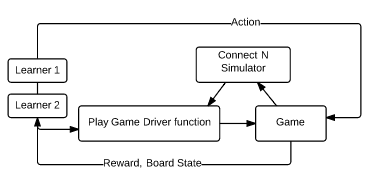
\includegraphics[scale=.7]{game_process.png}

\section{detailed description of state and action space including features, table with explanations as to why you encoded the state and action space they way you did is sufficient- everyone (andre)}

\section{detailed description of your results/comparisons- everyone- wait for results}

\section{thorough description of why you got the results you did, a few pages- everyone- wait for results}


\section{Approaches}
\textbf{THIS IS COMBINED MOTIVATION FOR APPROACHES + DETAILED DESCRIPTION OF APPROACHES}

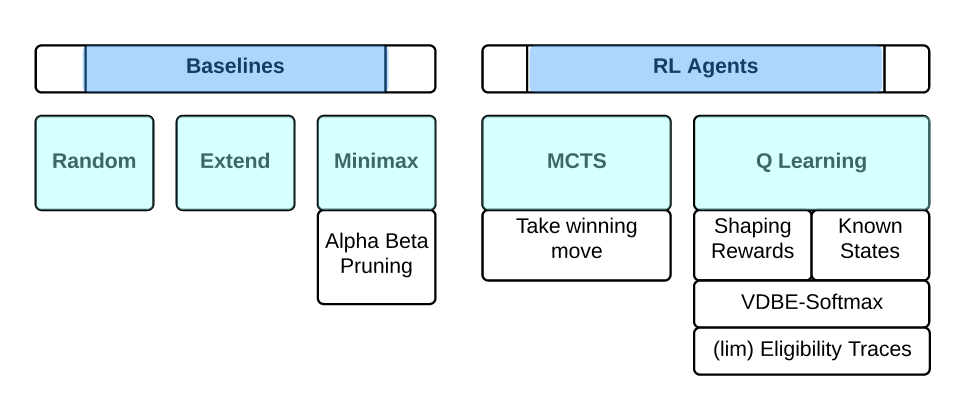
\includegraphics[scale=.4]{learners.png}

\subsubsection{Baselines} 

We implemented three baselines:
\begin{enumerate}
\item \textbf{Random action}, where the agent randomly chooses a column to put its token into at each time step
\item \textbf{Extend}, where the agent attempts to extend its largest current streak (horizontally, vertically, or diagonally), breaking ties between streaks randomly.
\item \textbf{Minimax}--- We implemented the Artificial Intelligence algorithm Minimax, which conceptualizes the Connect-N game as a tree of possible future game states. The current state of the game is the root node of the tree, and each of the children represent possible states resulting from a move that can be made from the current game state. The leaves are the final states of the game, or states where no further moves can be made because one player has one or lost. In traditional Minimax, leaves have a value of either positive infinity (win), negative infinity (lose), or 0 (tie), but such an algorithm forces Minimax to continue evaluating future board states until it reaches a win or a lose. However, this is often computationally infeasible as there are so many possible states in the game. Instead, we implement a \textbf{static evaluation} form of Minimax that takes a \textbf{depth} parameter that governs how far down the tree the algorithm should explore. We generate node values in Minimax according to this heuristic:

\begin{itemize}

\item For length of streak, each streak has value $x * 2^(x-1)$, where x is the length of the streak
\item For opponent streaks, each node has value $(x *  2^x) / 6$, where x is the length of the streak

We decided upon these values \textbf{LUCY}!!!!

\end{itemize}

We also explore an extension to Minimax, called \textbf{alpha-beta pruning}, motivated by the idea that often Minimax explores more branches than is required. For example, if it needs to expand down to depth 3, but is currently at depth 2, it will continue expanding all branches to depth 3 even if one branch clearly would lead to a loss. In alpha-beta pruned Minimax, the tree is pruned to only continue investigating good paths. The algorithm controls the range of values the tree should continue searching down, and we initialize this range to $\pm 1000$ for generality.

\end{enumerate}

\subsubsection{Q Learning}

The first reinforcement learning approach we looked at was Q Learning, an off-policy TD control algorithm that we investigated in Practical 1. The straightforward version of Q Learning we implemented in Practical 1 did not seem like it could have any chance of performing as well as an AI algorithm such as Minimax, so we additionally implemented a number of extensions to Q Learning.

\begin{enumerate}
\item We replaced $\epsilon$-greedy with the \textbf{VDBE-Softmax} policy described in [Tokic, 2011]. When evaluated on the Gridworld, VDBE-Softmax outperformed $\epsilon$-greedy in cumulative reward substantially, so we thought it could potentially do better in Connect-N as well.
\item We implemented \textbf{eligibility traces}, as described in the Sutton and Barto textbook and as we covered in class discussions, as it can help the learner learn more efficiently. Unfortunately, the complete eligibility traces algorithm iterates over all states and actions, which was computationally infeasible in this game, as the states represent all possible versions of the Connect N board state. Instead, we implement a limited version of eligibility traces, where the algorithm updates $Q(s, a)$ and $e(s, a)$ for each board state it currently knows and all board states that can be reached by taking one action from the current board state.
\item \textbf{LUCY}- add known states and shaping rewards

\end{enumerate}

\begin{wrapfigure}{l}{5cm}
	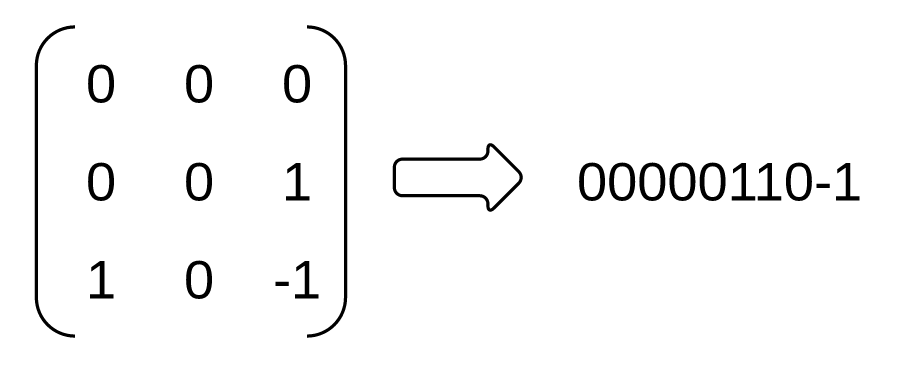
\includegraphics[scale=.16]{transform}
\end{wrapfigure}

The Q learner continues to keep an action value table (as in Practical 1), with a slightly different data structure. The Q learner takes the board state and hashes it into a string, where 0 represents an empty spot and 1 and -1 represent self and opponent tokens. It then adds the string board state as a key into a dictionary. For computational reasons, instead of adding all of the possible board states to the dictionary, the dictionary only ever holds board states that it has seen. 

To pre-train the Q learner, we pass the board state between different games, allowing the Q learner to have a better, more competitive knowledge of what actions are good or bad.

\subsubsection{Monte Carlo Tree Search- andre} 


\section{Future Work}

Interesting research questions for the future could include:

\begin{enumerate}
\item Exploring extensions to MCTS, such as a better default policy (perhaps estimation of a value for each board state, and selecting the action that leads to the board state with highest value)
\item Exploring large N, where computational complexity of solving MCTS and Minimax could potentially allow Q learning to perform competitively (as MCTS iteration number would be low and Minimax depth parameter would be low)
\item Adding stochasticity to the board, such as dropping the bottom row with some probability or having a probability of taking the wrong action
\item Coding the board state as a POMDP, with information such as the number of tokens in a row, but not knowing exactly where the tokens are 
\end{enumerate}


\end{document}







